\subsection{Server}

\subsubsection{Überblick}
\begin{figure}[h!]
    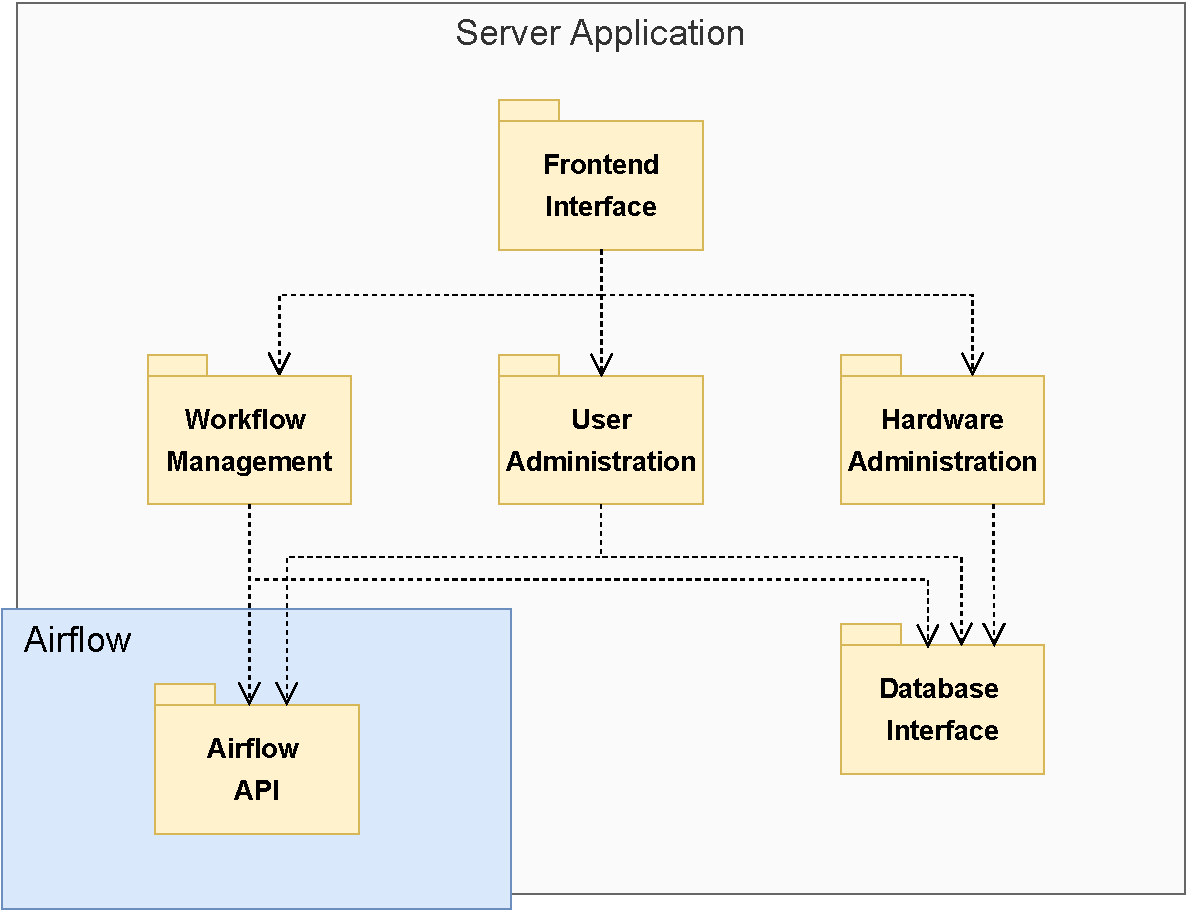
\includegraphics[width=1\textwidth]{res/Moduluebersicht.pdf}
    \caption{Übersicht über den Entwurf der Server Anwendung}
\end{figure}
Die Server Anwendung ist in ihren Grundzügen in einer Schichtenarchitektur aufgebaut. 
Die zentrale Anlaufstelle für Anfragen des Clients stellt das API Package dar.
Dieses hat Abhängigkeiten zu den Workflow, User Administration und Hardware Administration Packages, welche wiederum auf die Datenbank-Schnittstelle und die Airflow API zugreifen.

\FloatBarrier
\newpage

\subsubsection{\nameref{API}}
\begin{figure}[h!]
    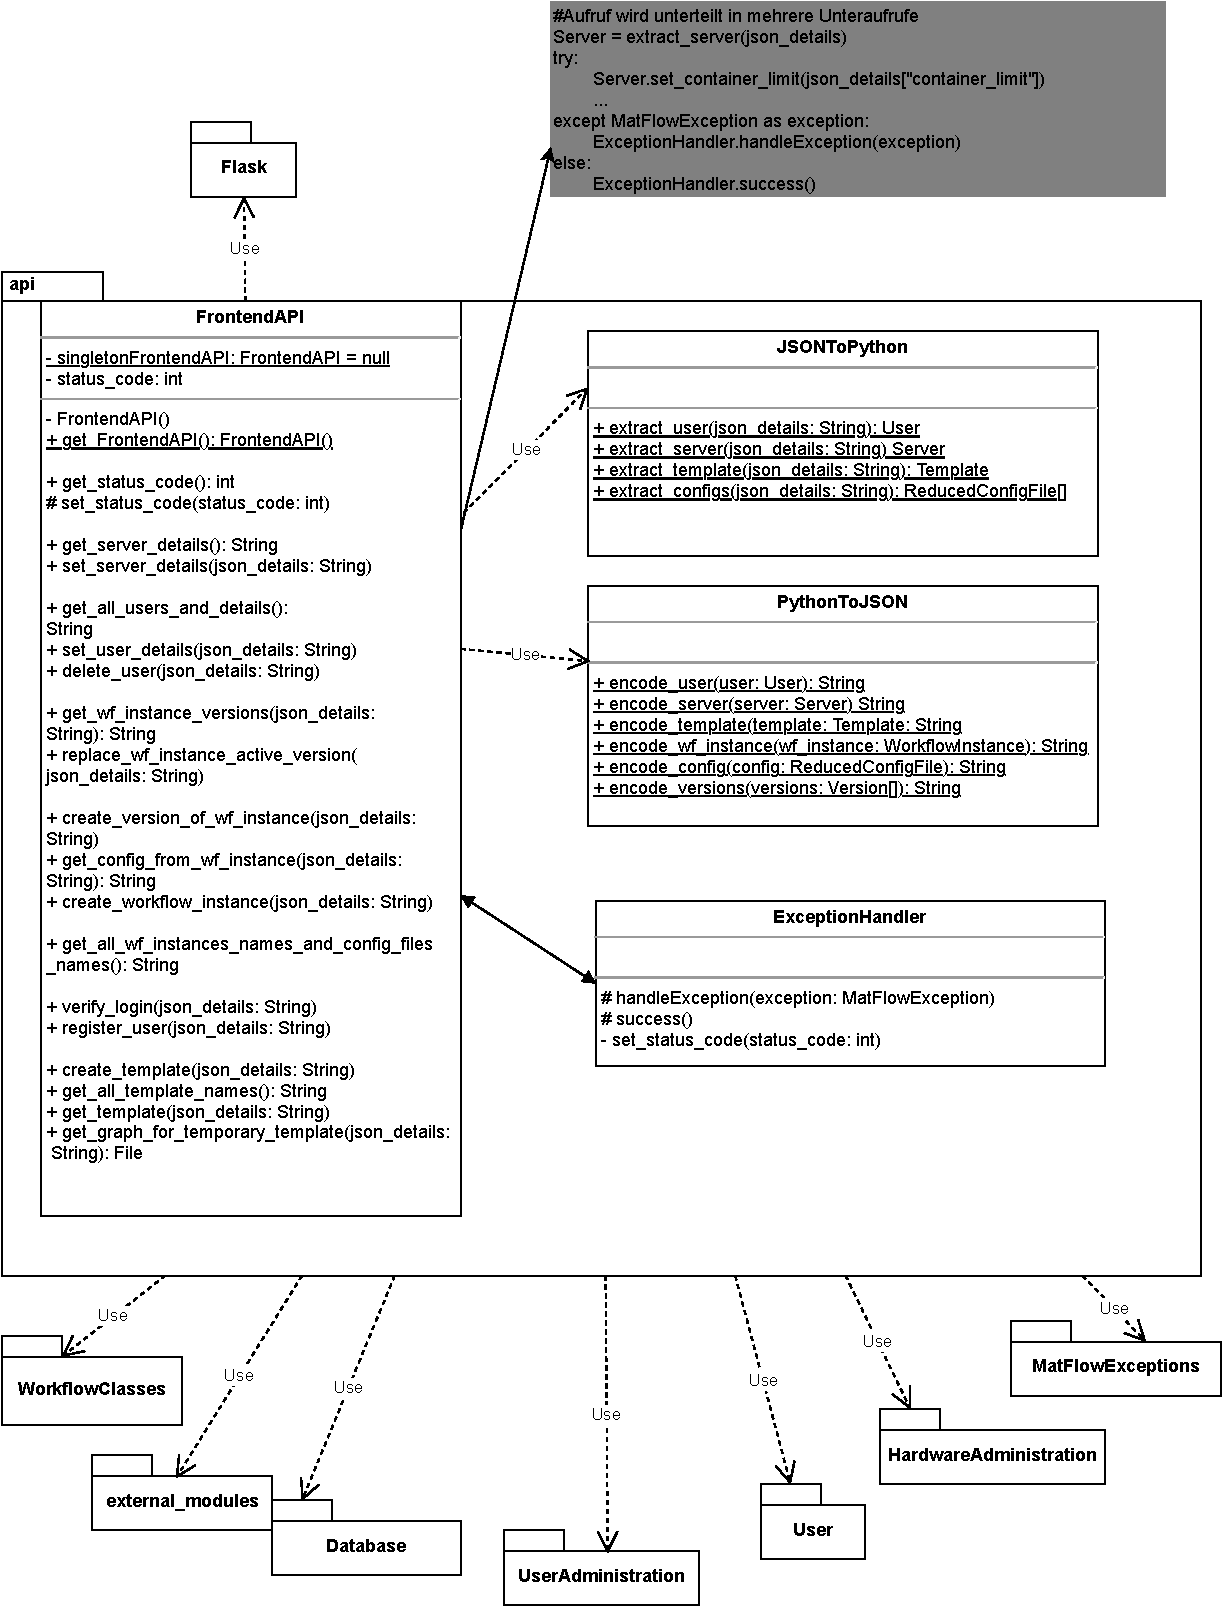
\includegraphics[width=0.85\textwidth]{res/api.drawio.pdf}
    \caption{API Package}
\end{figure}
\FloatBarrier
Dieses Package ist zuständig für die Kommunikation zwischen der Client Applikation und der Serverapplikation (siehe Kapitel 
Kommunikation). Anfragen an die Klasse FrontendAPI werden an die dementsprechenden packages weitergeleitet, wo diese konkret 
ausgeführt werden. Diese Klasse fängt alle Exceptions und leitet sie an die Klasse ExceptionHandler weiter.
In der ExceptionHandler Klasse wird dann der Status Code der FrontendAPI Klasse geändert, der für den Client aussagekräftig
darüber ist welcher Fehler geworfen wurde.


\newpage

\subsubsection{Workflow package}
\begin{figure}[h!]
    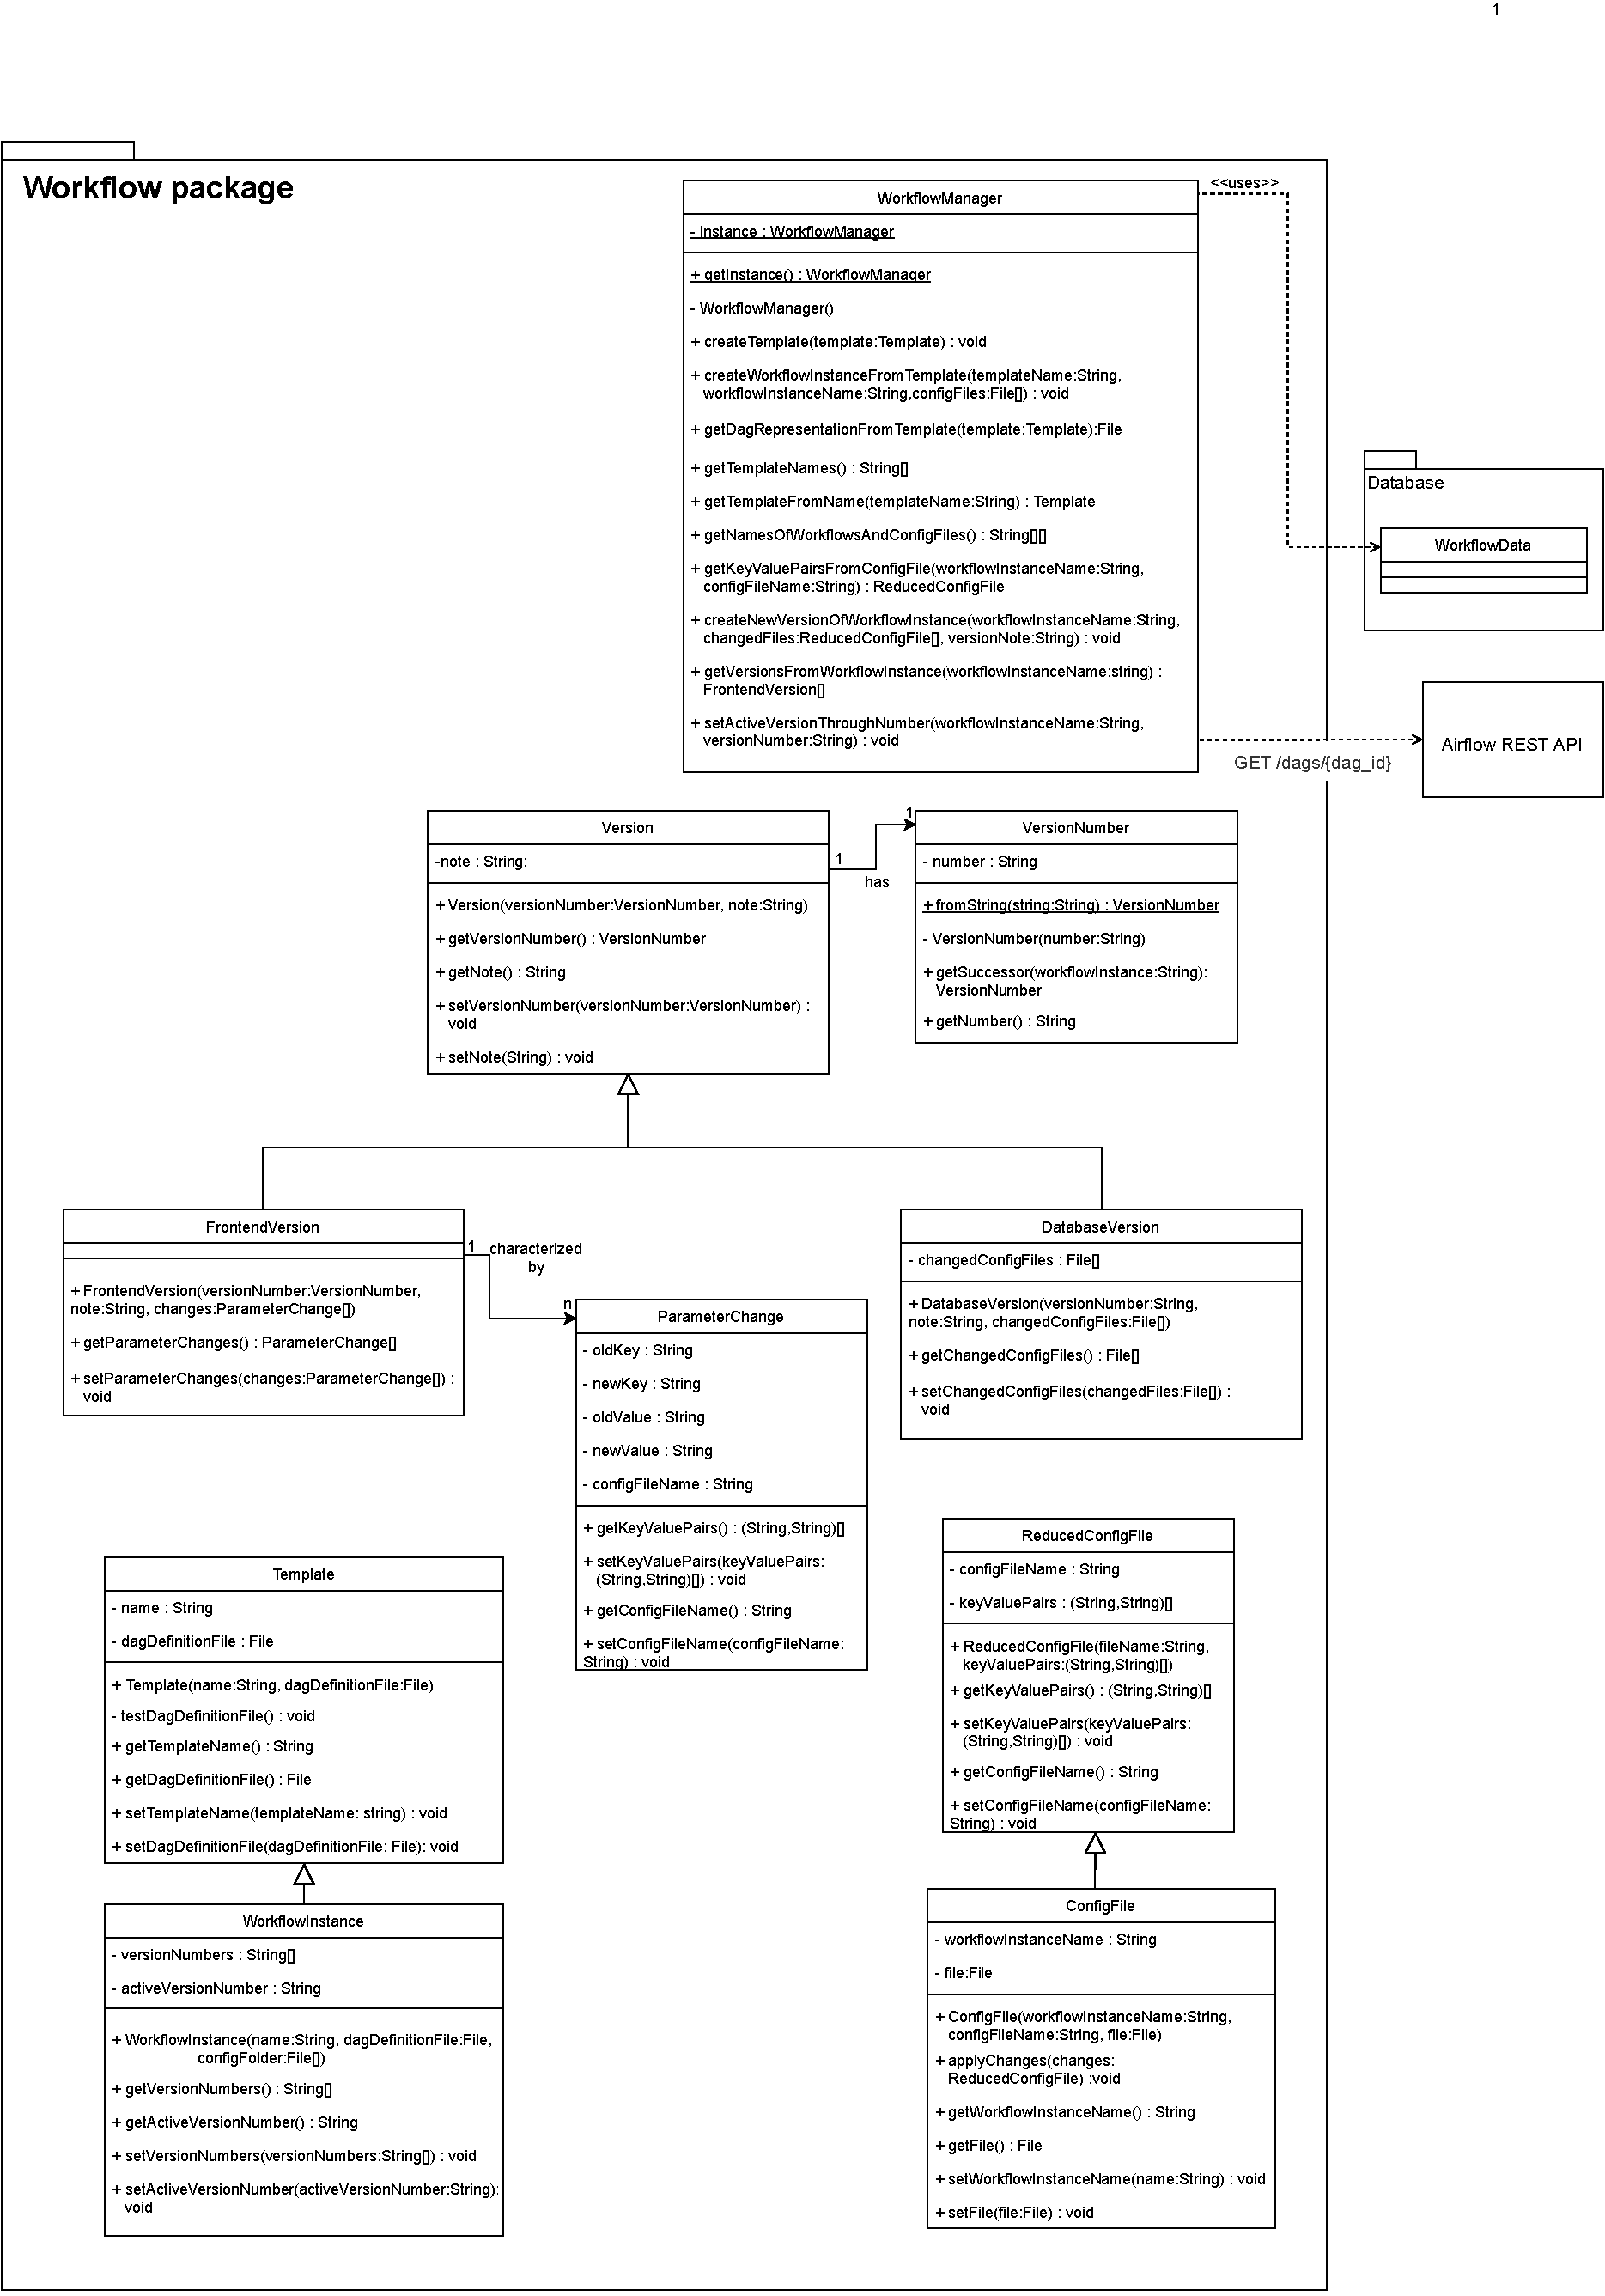
\includegraphics[width=0.85\textwidth]{res/Klassen/wfPackage.pdf}
    \caption{Klassendiagramm des Workflow packages}
\end{figure}
\FloatBarrier
Das Workflow Package ist für die Erstellung und Verwaltung von Workflow-Templates, -Instanzen und -Versionen zuständig.
Es stellt ein Bindeglied in der Kommunikationskette zwischen Client, Airflow und der Datenban dar.
Alle Anfragen die vom Client gestellt und der API weitergeleitet werden kommen zentral im Singleton-Objekt der Klasse WorkflowManager an.
Dieses erstellt dann andere Objekte und stellt seinerseits Anfragen an die Airflow API und die Datenbank-Schnittstelle.

\FloatBarrier
\newpage

\subsubsection{User Administration}
\begin{figure}[h!]
    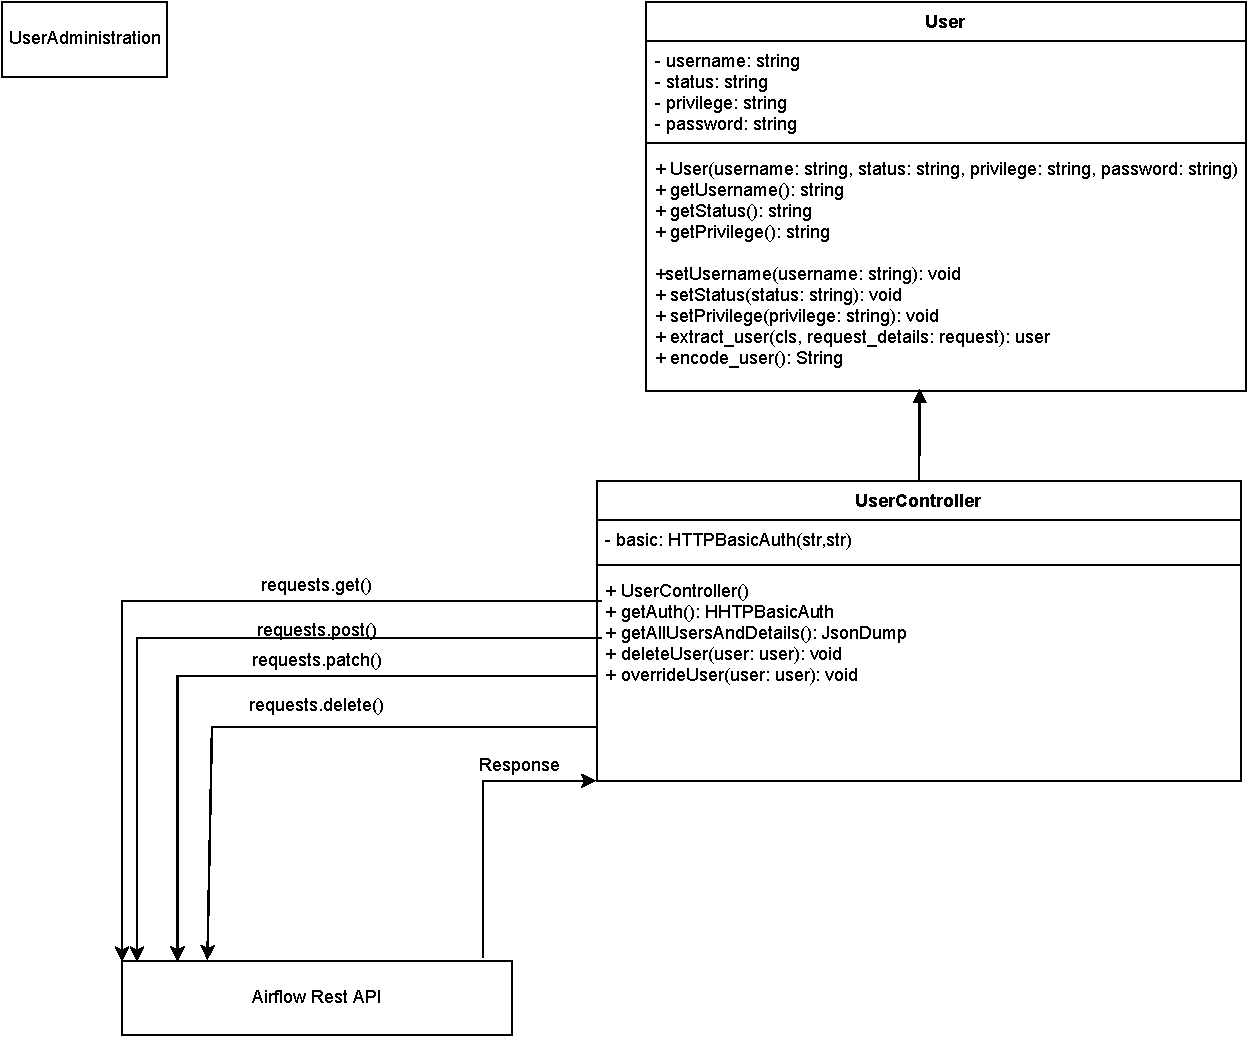
\includegraphics[width=1\textwidth]{res/UserAdministration.pdf}
    \caption{Klassendiagramm der User Administration}
\end{figure}
\FloatBarrier
Das User Administration Package ist für die Anlegung und Verwaltung von User-Accounts zuständig.
Dabei benutzt es die Airflow API, um User sowohl in der Anwendung, als auch in Airflow parallell zu verwalten.

\FloatBarrier
\newpage

\subsubsection{Hardware Administration}
\begin{figure}[h!]
    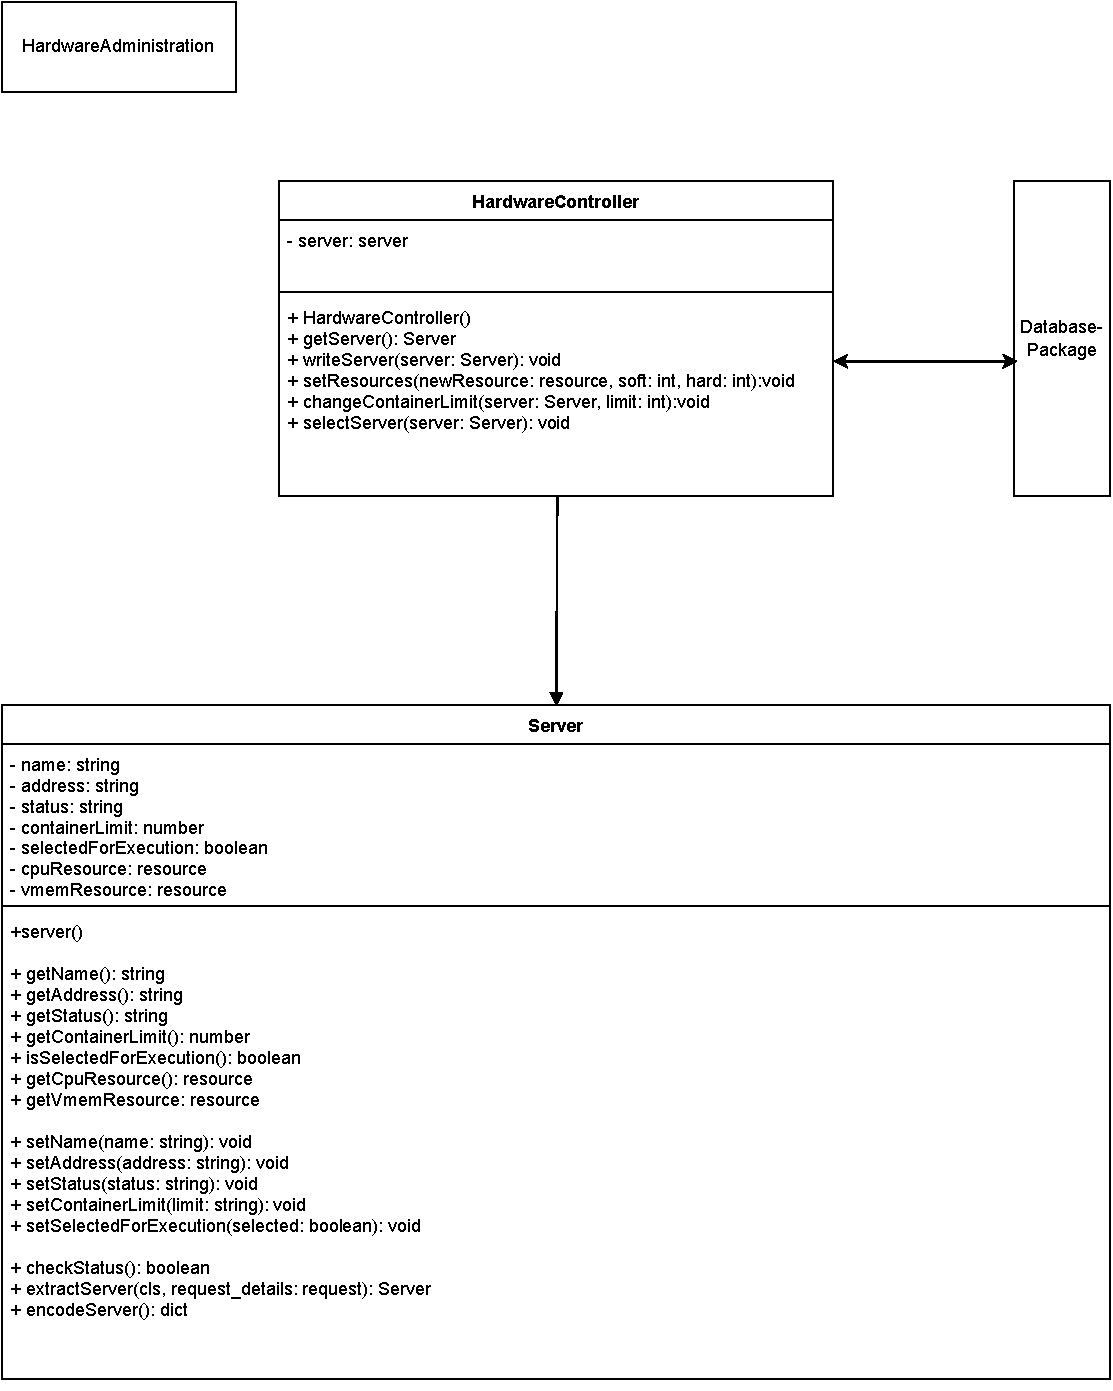
\includegraphics[width=1\textwidth]{res/HardwareAdministration.pdf}
    \caption{Klassendiagramm der Hardware Administration}
\end{figure}
\FloatBarrier
Das Hardware Administration Package ist für die Anlegung und Verwaltung von Servern zuständig.

\FloatBarrier
\newpage

\subsubsection{\nameref{database}}
\begin{figure}[h!]
	\centering
	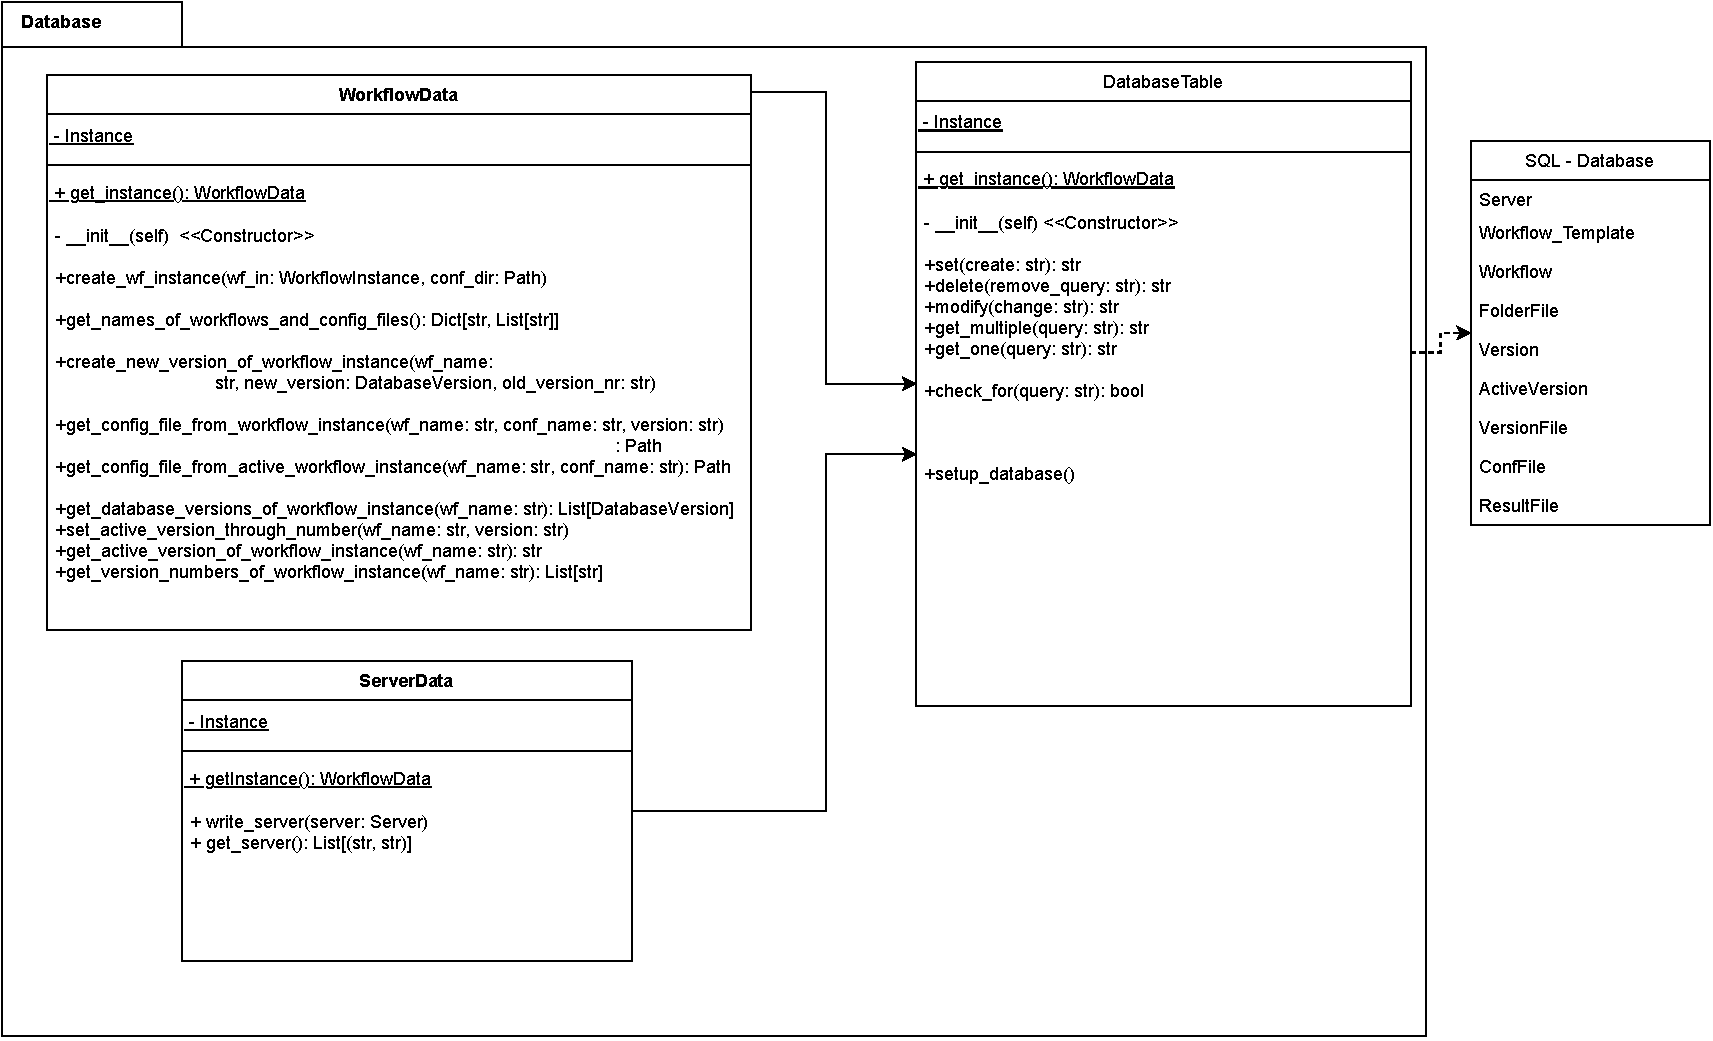
\includegraphics[width=1\textwidth]{res/Database_Package.pdf} 
	\caption{Klassendiagramm von Database}
	\label{fig:database_package}
\end{figure}

\FloatBarrier
Das Datenbank Package entwirft für einen Aufruf einer Funktion einer Klasse in diesem Package den entsprechenden SQL Ausdruck und ruft diesen auf der Datenbank auf.
Bei fehlerhaften Aufrufen, wie zum Beispiel der Abfrage eines Workflows der nicht existiert, wird eine entsprechende MathFlowException an den Aufrufer zurückgeworfen.

\newpage

\subsubsection{TGDSOperator}
\begin{figure}[h!]
    \centering
    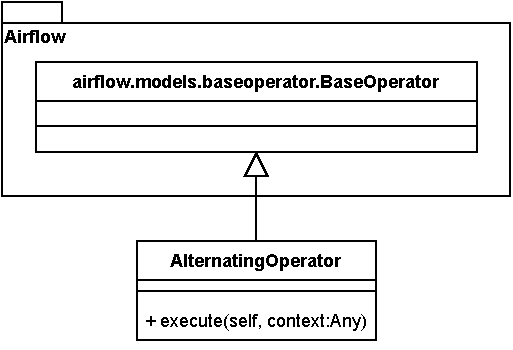
\includegraphics[width=0.65\textwidth]{res/Klassen/tgdsOp.pdf}
    \caption{Klassendiagramm des TGDS-Operators}
\end{figure}
\FloatBarrier
Die Aufgabe dieses Packages ist es Airflow um einen Operator, den AlternatingOperator, zu erweitern.
Der Operator kann dann verwendet werden um zwei Tasks im Wechsel auszuführen. 
Dies ist bei der Implementierung eines bestimmten Theory-Guided-Data-Science-Modells von Nutzen. 

\FloatBarrier
\newpage

\subsubsection{MatFlowExceptions}
\begin{figure}[h!]
    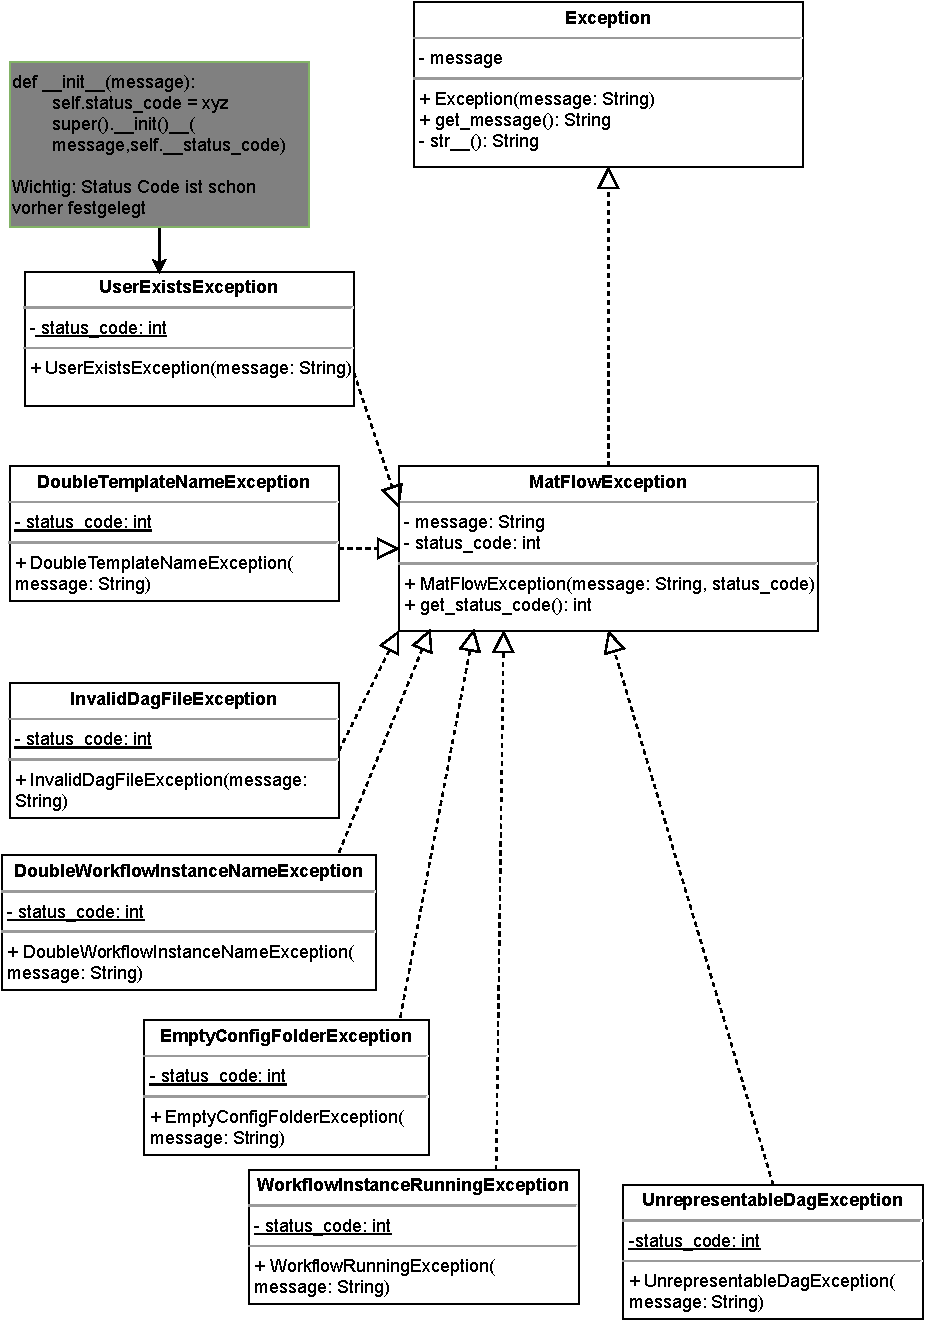
\includegraphics[width=0.8\textwidth]{res/Klassen/MatFlowExceptions.drawio.pdf}
    \caption{MatFlowExceptions}
\end{figure}
Dieses Package beinhaltet alle MatFlowExceptions. Diese werden geworfen, wenn es einen MatFlow spezifischen Fehler, ausgelöst 
durch den Nutzer, in der Anwendung gibt.

\FloatBarrier
\newpage